%
% This is a borrowed LaTeX template file for lecture notes for CS267,
% Applications of Parallel Computing, UCBerkeley EECS Department.
% Now being used for CMU's 10725 Fall 2012 Optimization course
% taught by Geoff Gordon and Ryan Tibshirani.  When preparing
% LaTeX notes for this class, please use this template.
%
% To familiarize yourself with this template, the body contains
% some examples of its use.  Look them over.  Then you can
% run LaTeX on this file.  After you have LaTeXed this file then
% you can look over the result either by printing it out with
% dvips or using xdvi. "pdflatex template.tex" should also work.
%

\documentclass[twoside]{article}
\setlength{\oddsidemargin}{0.25 in}
\setlength{\evensidemargin}{-0.25 in}
\setlength{\topmargin}{-0.6 in}
\setlength{\textwidth}{6.5 in}
\setlength{\textheight}{8.5 in}
\setlength{\headsep}{0.75 in}
\setlength{\parindent}{0 in}
\setlength{\parskip}{0.1 in}

%
% ADD PACKAGES here:
%

\usepackage{amsmath,amsfonts,graphicx,amsthm,amssymb}
\usepackage{hyperref}
\usepackage[ruled,vlined]{algorithm2e}
\usepackage{cancel}

\hypersetup{
    colorlinks=true,
    linkcolor=blue,
    filecolor=magenta,
    urlcolor=blue,
}

%
% The following commands set up the lecnum (lecture number)
% counter and make various numbering schemes work relative
% to the lecture number.
%
\newcommand*{\QEDB}{\hfill\ensuremath{\square}}%
\newcommand*\xor{\mathbin{\oplus}}
\newcounter{lecnum}
\renewcommand{\thepage}{\thelecnum-\arabic{page}}
\renewcommand{\thesection}{\thelecnum.\arabic{section}}
\renewcommand{\theequation}{\thelecnum.\arabic{equation}}
\renewcommand{\thefigure}{\thelecnum.\arabic{figure}}
\renewcommand{\thetable}{\thelecnum.\arabic{table}}

%
% The following macro is used to generate the header.
%
\newcommand{\lecture}[4]{
   \pagestyle{myheadings}
   \thispagestyle{plain}
   \newpage
   \setcounter{lecnum}{#1}
   \setcounter{page}{1}
   \noindent
   \begin{center}
   \framebox{
      \vbox{\vspace{2mm}
    \hbox to 6.28in { {\bf EE 381V: Special Topics on Unsupervised Learning
        \hfill Spring 2018} }
       \vspace{4mm}
       \hbox to 6.28in { {\Large \hfill Lecture #1: #2  \hfill} }
       \vspace{2mm}
       \hbox to 6.28in { {\it Lecturer: #3 \hfill Scribes: #4} }
      \vspace{2mm}}
   }
   \end{center}
   \markboth{Lecture #1: #2}{Lecture #1: #2}

   % {\bf Note}: {\it LaTeX template courtesy of UC Berkeley EECS dept.}

   % {\bf Disclaimer}: {\it These notes have not been subjected to the
   % usual scrutiny reserved for formal publications.  They may be distributed
   % outside this class only with the permission of the Instructor.}
   \vspace*{4mm}
}
%
% Convention for citations is authors' initials followed by the year.
% For example, to cite a paper by Leighton and Maggs you would type
% \cite{LM89}, and to cite a paper by Strassen you would type \cite{S69}.
% (To avoid bibliography problems, for now we redefine the \cite command.)
% Also commands that create a suitable format for the reference list.
\renewcommand{\cite}[1]{[#1]}
\def\beginrefs{\begin{list}%
        {[\arabic{equation}]}{\usecounter{equation}
         \setlength{\leftmargin}{2.0truecm}\setlength{\labelsep}{0.4truecm}%
         \setlength{\labelwidth}{1.6truecm}}}
\def\endrefs{\end{list}}
\def\bibentry#1{\item[\hbox{[#1]}]}

%Use this command for a figure; it puts a figure in wherever you want it.
%usage: \fig{NUMBER}{SPACE-IN-INCHES}{CAPTION}
\newcommand{\fig}[3]{
			\vspace{#2}
			\begin{center}
			Figure \thelecnum.#1:~#3
			\end{center}
	}
% Use these for theorems, lemmas, proofs, etc.
\theoremstyle{definition}
\newtheorem{theorem}{Theorem}[lecnum]
\newtheorem{example}{Example}
\newtheorem{lemma}[theorem]{Lemma}
\newtheorem{proposition}[theorem]{Proposition}
\newtheorem{claim}[theorem]{Claim}
\newtheorem{corollary}[theorem]{Corollary}
\newtheorem{note}{Note}
\newtheorem{definition}[theorem]{Definition}

% **** IF YOU WANT TO DEFINE ADDITIONAL MACROS FOR YOURSELF, PUT THEM HERE:

\newcommand\E{\mathbb{E}}
\newtheorem{problem}{Problem}
\DeclareMathOperator*{\argmax}{arg\,max}
\newenvironment{subproof}[1][\proofname]{%
  \renewcommand{\qedsymbol}{$\blacksquare$}%
  \begin{proof}[#1]%
}{%
  \end{proof}%
}
\allowdisplaybreaks


\begin{document}
%FILL IN THE RIGHT INFO.
%\lecture{**LECTURE-NUMBER**}{**DATE**}{**LECTURER**}{**SCRIBE**}
\lecture{7}{February 8th}{Professor Alex Dimakis}{Justin Lewis, Dany Haddad}
%\footnotetext{These notes are partially based on those of Nigel Mansell.}

% **** YOUR NOTES GO HERE:

% Some general latex examples and examples making use of the
% macros follow.
%**** IN GENERAL, BE BRIEF. LONG SCRIBE NOTES, NO MATTER HOW WELL WRITTEN,
%**** ARE NEVER READ BY ANYBODY.
This lecture's notes illustrate some uses of
various \LaTeX\ macros.
Take a look at this and imitate.

\subsubsection*{Topics Covered} % Don't be this informal in your notes!
\begin{itemize}
\item Submodularity
\item Feature selection (see \cite{KG05-1})
\item Nemhauser's proof for greedy maximization of submodular functions
\end{itemize}

\section{Definitions}

\subsubsection*{Entropy}
Given a set, $S$, of discrete random variables, define
the set function $f_H(S): 2^V \mapsto \mathbb{R}$
$$f_H(S) = H(X_S) = - \sum_{x_i \in S} p(x_i)\log p(x_i) $$
and for differential entropy:

$$f_H(S) = H(X_S) = - \int_{\mathcal{X}_S} p(x)\log p(x)dx $$

\subsubsection*{Mutual Information}
Given random vectors $Y$ and $X_S$, define the following as the mutual
information between them $f_I(S):~2^V~\mapsto~\mathbb{R}$
$$f_I(S) = I(Y; X_S) = H(Y) - H(Y | X_S)$$

\section{Properties}

\begin{lemma}
$f_H$ is submodular.
\end{lemma}

\begin{proof}
  Consider subsets $A$ and $B$ of random variables,
  $\mathcal{X}$, where $A \subseteq B$. Also consider a random
  variable $X_m \notin A \cup B$
  $$f_H(A \cup \{m\}) - f_H(X_A) = H(X_A, X_m) - H(X_A) = H(X_m | X_A)$$
  \centering and similarly
  $$f_H(B \cup \{m\}) - f_H(X_B) = H(X_m | X_B)$$
  Since conditioning on a larger set of random variables cannot
  increase the entropy:
  \begin{align*}
    H(X_m | X_B) & \leq H(X_m | X_A) \\
    f_H(B \cup \{m\}) - f_H(X_B) & \leq f_H(A \cup \{m\}) - f_H(X_A)
  \end{align*}
\end{proof}

% \begin{note}
%   $2^{H(X)}$ is the volume of the support set of $X$.
% \end{note}

In the discrete case we can show that $f_H$ is also monotone. Howevers,
in the continuous case, this function is no longer
monotone.\footnote{see Krause \& Golovia survey:
  \href{https://las.inf.ethz.ch/files/krause12survey.pdf}{https://las.inf.ethz.ch/files/krause12survey.pdf}}
(TODO: counterexample).

\begin{example}
  Consider $X_1, ..., X_n$ jointly gaussian random variables with pdf:
  $$p(x) = \frac{1}{\sqrt{2\pi |\Sigma|}} e^{-\frac{1}{2}(x-\mu)^T
    \Sigma^{-1} (x-\mu)}$$

  The differential entropy of a subset indexed by $S$ is given by:
  $$H(X_S) = \frac{1}{2} 2 \pi e\log \det \Sigma_s$$
  Where $\Sigma_S$ denotes the submatrix of the covariance matrix
  $\Sigma$ formed by taking only the variables indexed by $S$. So to
  choose the subset of $k$ variables with the largest entropy, we must
  maximize the determinant of $\Sigma_S$.
  \QEDB
\end{example}

\begin{proposition}
  Mutual information is, in general, not submodular.
\end{proposition}
\begin{proof}
  Consider $X$, $Y$
  independent $Bernoulli(\frac{1}{2})$ random variables. Let $Z = X
  \xor Y$. So:

  $$H(Z) = H (Z | X) = H (Z | Y) = 1  \text{ and } H (Z | X \cup Y) = 0$$
  $$\implies H(Z) - H(Z | X) \leq H (Z | Y) - H (Z | X \cup Y)$$
\end{proof}

\begin{claim}
  Mutual information is monotone. This follows immediately from
  the fact that conditioning does not increase entropy.
\end{claim}

\begin{proposition}
  TODO: fix this proof
  Given sets $S$ and $U$ of random variables such that the elements of
  $S$ are independent of each other conditioned on $X_U$, then $f_I(A) = I(U;
  A)$
  is submodular for all $A \subseteq S \cup U$.
\end{proposition}

\begin{proof}
  Let $W = U \cup S$ and $C = A \cup B$ such that $A, B \subseteq W$. So:
  \begin{align*}
    H (U | C) &= H (U |A \cup B) \\
              &= H (U \cup A) - H(A \cup B) \\
              &= H (A|U)+ H (U) - H (C) \\
              &= H (U) - H (C) + \sum_{Y \in C \cap S} H (Y |U)
  \end{align*}
  Where the last step follows using the chain rule for the joint entropy. H (U) is constant, H (C) is submodular and ∑ Y ∈C∩S H (Y | U) is linear in C on U ∪S and hence on W .
\end{proof}

\begin{figure}[h]
  \centering
  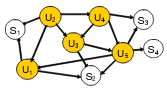
\includegraphics[scale=0.8]{cond_ind.png}
  \caption{An undirected graphical model where the elemets of $S$ are
    independent conditioned on $U$}
  \label{fig:ugm}
\end{figure}

This claim holds if the distribution factorizes according to an
undirected graphical model similar to \ref{fig:ugm}. Recall the conditional
independence properties we can infer from an undirected graphical
model.

\section{Optimization}

Consider the chain rule of entropy:
$$H(X_1, ..., X_n) = H(X_S) + H(X_{S^c} | X_S)$$
Since $H(X_1, ..., X_n)$ has no dependence on $S$, maximizing the
entropy of the subset $S$, is equivalent to minimizing the
uncertainty of the unobserved set, $S^c$:
$$\max_{s: |s| \leq k} H(X_S) = \min_{s: |s| \leq k} H(X_{S^c} |
X_S)$$
This requires us to maximize a monotone submodular function. The
greedy algorithm selects the element with the largest discrete
derivative at iteration $i$.


%----------------------------------------------------------------------------------------
%----------------------------------------------------------------------------------------

\section{Approx. Submodular Function Maximization}


It is well known that maximizing an arbitrary submodular function with
given constraint set is, in general, NP-Hard. %(REFERENCE?)

\begin{problem}
Given ground set $S_g$, subset $S \subseteq S_g$, and submodular set function $f(\cdot)$:

$\displaystyle \max_{S \, \subseteq \, S_g} f(S)$

$\text{subject to}$ $|S| \leq k$

\end{problem}

%To reiterate, there are a number of well known problems which reduce to submodular maximization (UNNECESSARY?):
%
%\begin{itemize}
%\item Max cut
%\item Max cover
%\item Sensor selection
%\item Knapsack problem
%\end{itemize}

Finding the optimal solution may be intractable; however, an approximate solution known as the Greedy Algorithm can achieve fair results. More specifically:

\begin{algorithm}[H]
\SetAlgoLined
\caption{Greedy Algorithm}
\SetKw{Kw}{Define}
\Kw{ground set $S_g$, subset $S \subseteq S_g$, set function $f(\cdot)$, and cardinality constraint $|S| \leq k$  }\;
\SetKw{Kw}{Description}
\Kw{ greedily add to $S$ at iteration $i$ the element with the largest discrete derivative}\;
\KwResult{$S_{greedy}$ }
 $S_0=\emptyset$\;
 \While{$|S_i| \leq k$}{
  $\displaystyle S_{i+1} = S_i \, \cup \, \argmax_{s \in \{S_g \diagup S_i\}} \bigg\{ \Delta(s\diagup S_i) \bigg\}$ \;
%  \eIf{condition}{
%   instructions1\;
%   instructions2\;
%   }{
%   instructions3\;
%  }
 }

\end{algorithm}

\newpage

\begin{theorem}
Let $S^*$ denote the optimal subset , and $S_{greedy,\ell}$ as the Greedy Algorithm selection after $\ell$ iterations. Given set function $f$ which is submodular, monotone, non-negative, and $f(\emptyset)=0$ :

$f(S_{greedy,\ell}) \geq [1-\text{exp}[-\dfrac{\ell}{k}]] \cdot f(S^*)$
	
$f(S_{greedy,\ell=k}) \geq [1-\dfrac{1}{e}] \cdot f(S^*) \approx 0.63 \cdot f(S^*)$

\end{theorem}

\begin{proof}
(Nemhauser and Wolsey) \footnote{see Nemhauser \& Wolsey survey:
  \href{http://www.cs.toronto.edu/~eidan/papers/submod-max.pdf}{http://www.cs.toronto.edu/~eidan/papers/submod-max.pdf}}

Let $S_i$ denote the Greedy algorithm selection after the $i$-th iteration

$f(S^*) \leq f(S^* \cup S_i)$ $\text{(monotonicity)}$

\begin{claim}
$\displaystyle f(S^* \cup S_i) = f(S_i) + \sum_{j=1}^{k} \Delta \bigg(v_j^* \diagup \big\{S_i \cup \{v_1^*,v_2^*,\ldots,v_{j-1}^*\}\big\}\bigg)$

\begin{subproof}[Subproof]
Expand:
%%%%
\begin{flalign*}
\displaystyle f(S^* \cup S_i) &= f(S_i) + \Delta \big(v_1^* \diagup S_i \big)
+\Delta \bigg(v_2^* \diagup \big\{S_i \cup v_1^*\big\}\bigg) 
+\cdots 
+\Delta \bigg(v_k^* \diagup \big\{S_i \cup \{v_1^*,v_2^*,\ldots,v_{k-1}^*\}\big\}\bigg) &\\
%%%%
&= \cancel{f(S_i)} + \cancel{{f(S_i \cup v_1^*)}} - \cancel{{f(S_i)}}
+ \cdots + f(S_i \cup \{v_1^*,v_2^*,\ldots,v_{k}^*\}) 
-\cancel{f(S_i \cup \{v_1^*,v_2^*,\ldots,v_{k-1}^*\})}  &\\
%%%%
&= f(S^* \cup S_i)
\end{flalign*}

The telescoping sum leaves only the desired term.

\end{subproof}
\end{claim}
%%%%
With claim above it follows: %%REFERENCE step 1?
%%%%
\begin{flalign*}
f(S^*) \leq f(S^* \cup S_i) &=  f(S_i) + \sum_{j=1}^{k} \Delta \bigg(v_j^* \diagup \big\{S_i \cup \{v_1^*,v_2^*,\ldots,v_{j-1}^*\}\big\}\bigg) & &\\
&\leq f(S_i) + \sum_{j=1}^{k} \Delta (v_j^* \diagup S_i) &\text{(by submodularity)} &\\
&\leq f(S_i) + \sum_{j=1}^{k} [f(S_{i+1})-f(S_i)] & \text{(by Greedy selection)} &\\
&= f(S_i) +k\cdot[f(S_{i+1})-f(S_i)]&\\
&\\
\Rightarrow f(S^*)-f(S_i) &\leq k\cdot[f(S_{i+1})-f(S_i)] &\\
\delta_i &\leq k\cdot[\delta_i-\delta_{i+1}] &(\delta_i \triangleq f(S^*)-f(S_i)) &\\
\delta_{i+1} &\leq (1-\dfrac{1}{k})\cdot\delta_i &\\
\delta_\ell &\leq (1-\dfrac{1}{k})^\ell\cdot\delta_0 &\\
&\\
f(S_\ell) &\geq (1-(1-\dfrac{1}{k})^\ell)\cdot f(S^*) 
&(\delta_0 = f(S^*)-f(\emptyset)=f(S^*) &\\
f(S_\ell) &\geq (1-\text{exp}(-\dfrac{\ell}{k}))\cdot f(S^*)
&(1-x \leq \text{exp}^{-x} \,\, \forall \, x) &\\
\end{flalign*}
\end{proof}



%----------------------------------------------------------------------------------------
%----------------------------------------------------------------------------------------




\subsection{latex reference}

Here is an itemized list:
\begin{itemize}
\item this is the first item;
\item this is the second item.
\end{itemize}

Here is an enumerated list:
\begin{enumerate}
\item this is the first item;
\item this is the second item.
\end{enumerate}

Here is an exercise:

{\bf Exercise:}  Show that ${\rm P}\ne{\rm NP}$.

Here is how to define things in the proper mathematical style.
Let $f_k$ be the $AND-OR$ function, defined by

\[ f_k(x_1, x_2, \ldots, x_{2^k}) = \left\{ \begin{array}{ll}

	x_1 & \mbox{if $k = 0$;} \\

	AND(f_{k-1}(x_1, \ldots, x_{2^{k-1}}),
	   f_{k-1}(x_{2^{k-1} + 1}, \ldots, x_{2^k}))
	 & \mbox{if $k$ is even;} \\

	OR(f_{k-1}(x_1, \ldots, x_{2^{k-1}}),
	   f_{k-1}(x_{2^{k-1} + 1}, \ldots, x_{2^k}))
	& \mbox{otherwise.}
	\end{array}
	\right. \]

\begin{theorem}
This is the first theorem.
\end{theorem}

\begin{proof}
This is the proof of the first theorem. We show how to write pseudo-code now.
%*** USE PSEUDO-CODE ONLY IF IT IS CLEARER THAN AN ENGLISH DESCRIPTION

Consider a comparison between $x$ and~$y$:
\begin{tabbing}
\hspace*{.25in} \= \hspace*{.25in} \= \hspace*{.25in} \= \hspace*{.25in} \= \hspace*{.25in} \=\kill
\>{\bf if} $x$ or $y$ or both are in $S$ {\bf then } \\
\>\> answer accordingly \\
\>{\bf else} \\
\>\>    Make the element with the larger score (say $x$) win the comparison \\
\>\> {\bf if} $F(x) + F(y) < \frac{n}{t-1}$ {\bf then} \\%
\>\>\> $F(x) \leftarrow F(x) + F(y)$ \\
\>\>\> $F(y) \leftarrow 0$ \\
\>\> {\bf else}  \\
\>\>\> $S \leftarrow S \cup \{ x \} $ \\
\>\>\> $r \leftarrow r+1$ \\
\>\> {\bf endif} \\
\>{\bf endif}
\end{tabbing}

This concludes the proof.
\end{proof}


\section{Next topic}

Here is a citation, just for fun~\cite{CW87}.

\section*{References}
\beginrefs
\bibentry{KG05-1}{\sc Krause, Andreas and Guestrin, Carlos},
``Near-optimal sensor placements,''
{\it Proceedings of the fifth international conference on Information
  processing in sensor networks - IPSN 06}, 2005.

\bibentry{KG05-2}{\sc Krause, Andreas and Guestrin, Carlos},
``Near-optimal Nonmyopic Value of Information in Graphical Models,''
{\it Proceedings of the Twenty-First Conference on Uncertainty in Artificial Intelligence}, 2005.
\endrefs

% **** THIS ENDS THE EXAMPLES. DON'T DELETE THE FOLLOWING LINE:

\end{document}
